\subsection{How to lay out elements}

Layout is always an important factor when using a visual language. A well laid out diagram is easier to understand and by centralizing important elements or
clustering related elements, you can actually impart additional information via a well-chosen layout.

\begin{enumerate}
\item[$\blacktriangleright$] To lay out a group of elements select them by drawing a selection box around them (or select them one by one by holding down
\texttt{Ctrl} and clicking on each element).

\begin{figure}[htbp]
\begin{center} 
  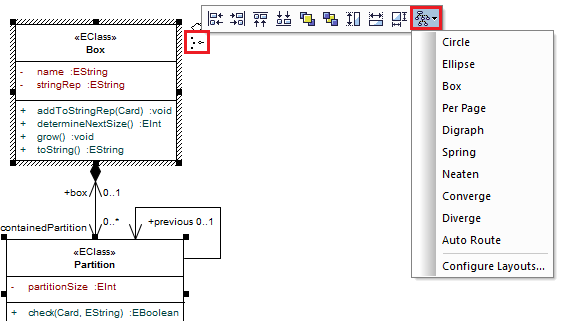
\includegraphics[width=0.85\textwidth]{layoutElements1}
  \caption{How to layout elements}  
  \label{fig_layout01}
\end{center}
\end{figure}
 
\item[$\blacktriangleright$] At the right side of the element that was selected last, a little symbol appears (Fig.~\ref{fig_layout01}). Click on the symbol to
obtain different options that are applied to all selected elements simultaneously. Experiment a bit to find out what effect each option has. The last symbol
opens a further drop-down menu with standard layout algorithms.

\newpage

\item[$\blacktriangleright$] Right-clicking one of the selected elements opens a different menu with a further set of layout options (Fig.~\ref{fig_layout02}).
\texttt{Align Centers} can be especially useful.

\begin{figure}[htbp]
\begin{center}  
  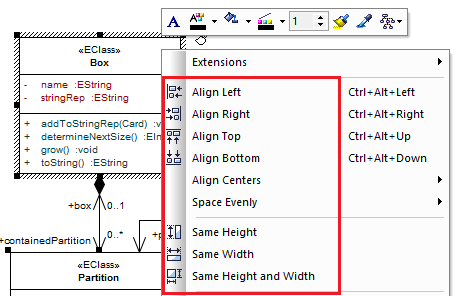
\includegraphics[width=0.85\textwidth]{layoutElements2}
  \caption{Further layout options}  
  \label{fig_layout02} 
\end{center}
\end{figure}

\end{enumerate}
